\section{Introduction}
Online tools increasingly use the wisdom of crowds to improve user experience.
For example, user-submitted product reviews in an e-commerce site can help recommend products to similar future users.
In these tools, users are not only consumers of the content but they also help create it.
The created content, like traditional surveys, are subject to a variety of biasing tendencies which have been well studied in the context of surveying methods \cite{groves2013survey}.

We explore a class of biases, collectively called \emph{Social Influence Bias}, which are biasing tendencies that arise from feedback from the community \cite{demarzo2003persuasion, moscovici1972social, wood2000attitude}.
One aspect of Social Influence Bias is the phenomenon called \emph{social herding}, where the feedback from the community encourages future participants to conform to what they perceive as the ``norm" in the community.
An application of particular interest is online participatory democracy where building and maintaining an online community are often cited as an advantage over traditional opinion polling as they increase the transparency of the system \cite{albors2008new,o2012transparency,noveck2008wiki}.
Understanding the effects of social herding is crucial to the design of recommendation algorithms as many of these algorithms rely on statistical independence assumptions and the spatial relationships between participant's features.

\begin{figure}[h]
  \centering
    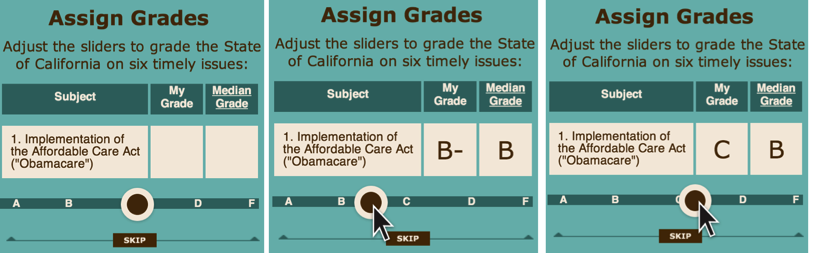
\includegraphics[width=\columnwidth]{../plots/grading-desc-1.png}
      \caption{Grading in the California Report Card. Participants enter grades on six timely issues facing the State of California. After entering their grades, the median grade over all participants is revealed. Participants have the option to change their grades after seeing the median. We model the tendency to regress towards the medians.}
      \label{grading-1}
\end{figure}

A common type of community feedback is revealing aggregate statistics (eg. show the average rating for a product) before a participant shares his or her opinion.
In this work, we specifically look at the biasing effect of showing aggregate statistics to participants.
In recent related work, Muchnik et al. \cite{muchnik2013social}, used a randomized experiment to determine the magnitude of social herding in up-voting in Reddit.com.
They randomly treated forum posts with extra up-votes and down-votes and measured the treatment effect; concluding that a statistically significant social herding tendency exists.
In this paper, we explore a related problem of whether participants will actually change their submissions upon revealing an aggregate statistic after they submit their input.
As a case study, we use the California Report Card \cite{crc}, where participants graded the state of California on six timely issues.
After submitting a grade, participants were shown the \emph{median} grade of all other participants.
We recorded any changes to previous grades that happened after the median was visible.

The findings of Muchnik et al. would suggest that we too will observe a biasing tendency in the form of a regression towards the observed median grade.
They, however, explored this question only on a binary input mechanism (up or down vote) and we extend this analysis to grading sliders with 13 possible vales from (A+ to F).
We further model this problem non-parametrically to make as few assumptions about the underlying distriubtion of grades.
In addition, our data was not collected in a randomized experiment like Muchnik et al.
Consequently, we had to design a hypothesis testing method based on Wilcoxon rank-sum test \cite{lehmann2006nonparametrics} to determine whether there was a significant regression towards the median grades that also mitigated the effects of some of the confounding variables.
We also those compare the results to a randomized online survey through SurveyMonkey.
We also devise a test that considers the consider the question of sequence-dependence, ie. whether the order of questions matters. 

In addition to the hypothesis testing, we fit models to the regression and its effects.
We use an information theoretic criteria to fit a flexibile degree polynomial to model the regression.
We also model how much more tightly centered around the median grade the changed grades are.

Our results suggest the following:
\begin{itemize}
\item There is a statistically significant regression towards the median for all of the issues.
\item The grades are statistically significantly more concentrated around the median in comparision to a reference survey.
\item For 4 out of the 6 issues, this regression can be modeled as linear in the difference between the participant's initial grade and the median.
\item For the other two issues, we found that the relationship can be modeled as a quadratic with greater regression for initial grades above the median.
\item Our sequence dependence results suggest a relationship, however, this was not statistically significant.
\end{itemize}
